\documentclass[10pt,a4paper]{article}
\usepackage{amssymb,amsmath}
\usepackage{cite}
\usepackage[pdftex]{graphicx}
\DeclareGraphicsExtensions{.jpg,.png}



\begin{document}
\title{Ass5 Solutions}
\author{Chang Li}
\maketitle

\section{Solutions}

\subsection{Linear Programming}

\begin{figure*}
	\centering
	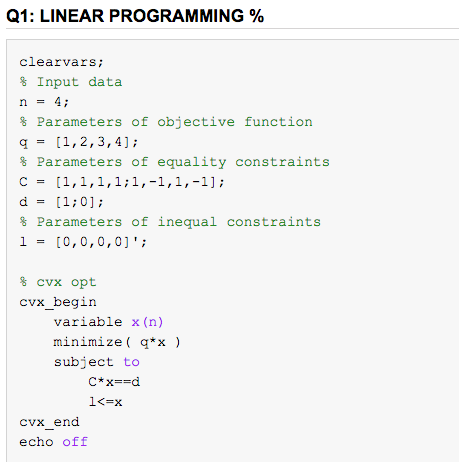
\includegraphics[width=0.7\linewidth]{images/Q1_code.png}
	\caption{"fawe"}
	\label{fig:code:Q1}
\end{figure*}


\subsection{Regularized Maximum Likelihood Estimation}

\subsubsection{a}
Because dataset $D$ is drawn from a Gaussian distribution
with mean $\mu$ and covariance $\Sigma$. Suppose $x\in R^n$,
so the density is:
$$p(x) = (2\pi)^{-n/2}det(\Sigma)^{-1/2}exp(-(x-\mu)^T\Sigma^{-1}(x-\mu)/2)$$
The average log-likelihood function has the form:
\begin{align*}
  l(D) & = E(\text{log}\;p(x_1,x_2,\dots,x_m))\\
       & = E(-\text{log}\;(2\pi) - \text{log}\;det\Sigma
  - \sum_{i=1}^{M}(-(x_i-\mu)^T\Sigma^{-1}(x_i-\mu)))
\end{align*}
Since $(x-\mu)^T\Sigma^{-1}(x-\mu)$ is a number and
$\mathrm{trace}(AB)=\mathrm{trace}(BA)$ therefore,
$$(x-\mu)^T\Sigma^{-1}(x-\mu)= \mathrm{tr}((x-\mu)^T\Sigma^{-1}(x-\mu))=\mathrm{tr}(\Sigma^{-1}(x-\mu)^T(x-\mu))$$ 
Plugging into expectation we get:
\begin{align*}
E[(x-\mu)^T\Sigma^{-1}(x-\mu)] &= E[\mathrm{tr}((x-\mu)^T(x-\mu)\Sigma^{-1}] )] \\
&= \mathrm{tr}(E[(x-\mu)^T(x-\mu)\Sigma^{-1}])\\
&= \mathrm{tr}(\hat{\Sigma}\Sigma^{-1})
\end{align*}
Plugging into the third term of $l(D)$ we can reformulate it as:
\begin{align*}
     l(D) &=- \text{log}\;det\Sigma - tr(\hat{\Sigma}\Sigma^{-1} )+ const \\
       & = \text{log}\;det\Sigma^{-1} - tr(\hat{\Sigma}\Sigma^{-1} ) + const 
\end{align*}

\subsubsection{b}
Because $K\succ 0$, we use the fact in section
3.1.5\cite{boyd2004convex} that the log of determinant is
concave so its negation is convex and
$\mathrm{tr}(\hat{\Sigma}K)$ is also convex. And the
absolute value function and summation operation are also
convex operations. Therefore the regularized maximum likelihood
optimization problem is a summation of convex functions and
henceTotal Variation Denoising convex.

\subsubsection{c}

\subsection{Total Variation Denoising}
For this question we are looking for a convex optimization problem. You do not need to give a closed-form solution.


	\renewcommand\refname{Bibliography}
	\bibliographystyle{ieeetr}
	\bibliography{ass5_ChangLi}
\end{document}
